\section{Introduction aux bandes}
Le plus gros du morceau arrive lorsque l'on s'intéresse à la représentation
réelle du document que l'on souhaite imprimer. Dans un premier temps,
l'étude de la représentation sera faite (dans cette section même) pour
embrayer ensuite sur les différents algorithmes de compression des
<< bandes >>.

\subsection{Du document à une carte de points}

\noindent\textit{\underline{Note : }La présente étude ayant été faite sur une
imprimante noir et blanc, il ne sera question que de ce type d'impression.}
\medskip

À la différence des langages comme le \emph{PostScript}, qui sont des langages
de dessins vectoriels, le QPDL est un langage qui décrit des images point
par point.

Pour pouvoir imprimer un document, il est alors nécessaire de le convertir
en une image où chaque bit correspond à un point sur la feuille. Le format
le plus proche de celui qui est compris par l'imprimante est le format
PBM\footnote{Portable BitMap}.

Pour rappel, le format PBM décrit, sans compression, une image bit par bit.
Un bit à un correspond à un point noir tandis qu'un bit à zéro correspond à
un point blanc. Les bits les uns à côté des autres représentent une ligne et
l'octet qui suit la fin d'une ligne débute la nouvelle ; et ce jusqu'à la fin
du document.

\subsection{De l'image d'une page à une bande}

Une fois le document converti en image, il est nécessaire de le découper en
bande. Les bandes représentent un nombre fini de lignes de points : une bande
représente exactement \emph{128 lignes} (soit $0x80$).

\subsection{Une vision par colonne}

À la différence d'une image PBM qui décrit une image ligne par ligne,
l'imprimante s'attend à ce que bandes représentent l'image \emph{colonne
par colonne}. De fait, le premier octet représente le premier octet de la
première ligne, le second octet représente le premier octet de la seconde
ligne, \ldots. Puis le 129\ieme{} octet représente le second octet de la
première ligne.

La figure \ref{fig:bande} représente ce traitement.

\begin{figure}[ht]
\centering
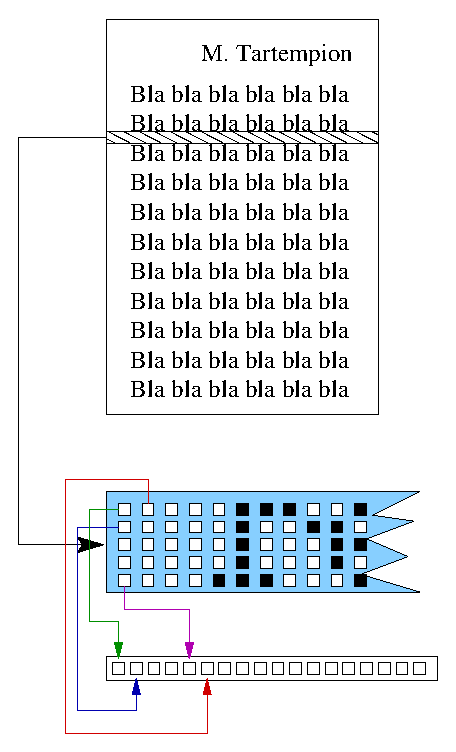
\includegraphics{Images/bande.eps}
\caption{Du document aux données réarrangées}
\label{fig:bande}
\end{figure}

\subsection{L'inversion des bits}
Alors que dans le fichier PBM, un bit monté correspondait à un point noir, 
pour l'imprimante c'est l'inverse. Il est donc indispensable d'appliquer
l'opérateur \emph{NON} à chaque octet de la bande.

\section{L'en-tête d'une bande}

Pour pouvoir convenablement réceptionner la bande et reformer le document,
un en-tête donne de précieuses indications comme le montre la table
\ref{tab:entete_bande}.

\begin{table}[!ht]
\centering
\begin{tabular}{| c | c | c |}
\hline
\textbf{Adresse} & \textbf{Description} & \textbf{Type} \\
\hline
\hline
0x0 & Valeur fixe $0xC$ & Octet \\
0x1 & Numéro de la bande & Octet \\
0x2 & Largeur de la bande & 16-Bits BE \\
0x4 & Hauteur de la bande & 16-Bits BE \\
0x6 & Version de la compression $0x11$ (?) & Octet \\
0x7 & Taille des données qui suivent & 32-Bits BE \\
\hline
\end{tabular}
\caption{En-tête d'une bande}
\label{tab:entete_bande}
\end{table}

\section{La compression des bandes}
Pour alléger la quantité de données transitant vers l'imprimante, les
données des bandes sont compressées. Il semble exister plusieurs versions
de l'algorithme de compression mais la description suivante ne touche
qu'à celle qui semble majoritairement utilisée : la version
\textsc{$0x11$}.

\subsection{L'en-tête des données compressées}
Pour pouvoir décompresser les données, des informations indispensables
sont données au travers d'un en-tête dont la description se trouve
dans la table \ref{tab:entete_compression}. À la différence des autres
en-têtes, celui-ci peut être écrit sans s'occuper de savoir si la
machine est en mode \emph{petit-boutien}\footnote{little-endian} ou
\emph{gros-boutien}\footnote{big-endian}. En effet, lorsque la
signature de l'en-tête est écrite ($0x9ABCDEF$), l'imprimante détecte
le type des prochaines données. Il suffit donc d'écrire naturellement
les données sans plus de tracas.

\begin{table}[!ht]
\centering
\begin{tabular}{| c | c | c |}
\hline
\textbf{Adresse} & \textbf{Description} & \textbf{Type} \\
\hline
\hline
0x0 & Valeur fixe $0x9ABCDEF$ & 32-Bits \\
0x4 & Taille données brutes ($ \leq 128$) & 32-Bits \\
0x8 & Table de pointeurs & 64 entrées de 16-Bits \\
0x88 & Début des données brutes & Variable \\
Variable & Données compressées & Variable \\
\hline
\end{tabular}
\caption{En-tête des données compressées}
\label{tab:entete_compression}
\end{table}

La signification des diverses entrées apparaîtra par la suite.

\subsection{L'algorithme de compression}
L'algorithme de compression vise à rechercher et à réduire des séquences
d'octets similaires. Pour ce faire, une \emph{table de pointeurs} de $64$
entrées va être dressée, puis le début des données va être recopié
en brut. Ensuite, pour chaque entrée de la table, on va comparer les
prochaines données à compresser avec celles pointées, relativement à la
position courante. La séquence pointée qui offre la meilleure
représentation sera gardée. Alors le numéro du pointeur avec la taille de
la séquence représentée sera inscrite. En revanche, si aucune séquence
n'arrive a représenter les prochaines données, celles-ci seront écrites
en brut jusqu'à trouver des données qui peuvent être représentée par une
séquence pointée par l'un des pointeurs de la table.

\subsection{La compression par un exemple}
L'étude d'un exemple concret permettra une meilleure compréhension. Soit une
table de 4 entrée :
\begin{exemple}
Tableau = \{-1; -3; -4; -5\}
\end{exemple}

et les données brutes suivantes :
\begin{exemple}
01 04 03 06 08 0F 0F 0F 0F 04 02 05 08 01 06 03 06 01 06
\end{exemple}

Les données suivantes sont à compresser :
\begin{exemple}
0F 0F 01 04 03 06 0F 01 04 05 06 0F 01 04 05 06 0F 0F 0F 0F 0F
\end{exemple}

Pour trouver la meilleure séquence, il faut passer en revue chacun des
pointeurs. Ceux-ci étant par rapport à la position actuelle, en prenant
le premier pointeur, la comparaison se fait entre 06 et 0F. La comparaison
s'arrête donc là. On remarque que pour les trois autres pointeurs, aucune
séquence n'est identique. Alors $0F$ sera écrit en brut dans les données.

Pour le second caractère, le premier pointeur est valable pour une longueur
de un ; et c'est le seul pointeur qui correspond. Malheureusement, si la
longueur de la séquence est \emph{inférieure à 3}, la compression n'est pas
bénéfique. Il est alors préférable d'écrire les données telles quelles.

Cela est valable pour les quatre autres caractères. En revanche, pour ce qui
est du septième caractère, le quatrième pointeur révèle une séquence de trois
caractères.

Le caractère suivant sera écrit en brut tandis que le quatrième
pointeur représente, là encore, bien la séquence qui suit, d'une taille de
sept octets.

Enfin, pour la fin, le premier pointeur représente bien la séquence de quatre
octets.
\medskip

Pour résumer, les données à compressées peuvent être représentées comme suit :

\begin{exemple}
Données brutes : 0F 0F 01 04 03 06 \\
Pointeur 4, taille = 3 \\
Données brutes : 05 \\
Pointeur 4, taille = 7 \\
Pointeur 1, taille = 4
\end{exemple}


\subsection{Le codage de la compression}
Comme il a été vu lors de l'étude de l'en-tête, le tableau de pointeur y est
stocké. Chaque entrée représente le déplacement en valeur absolue. De ce fait,
pour représenter le pointeur $-1$, l'entrée sera $1$. À la suite de l'en-tête
se trouve le début des données en brut. La quantité de données représentées
est en rapport avec le plus grand des pointeurs (en valeur absolue). Si
celui-ci est plus petit que $128$, alors il y aura autant de données en brut
que sa valeur. En revanche, si sa valeur est plus grande que $128$, il n'y aura
que $128$ octets de recopiés en brut. Enfin, la quantité de données brutes
sera recopiée au bon emplacement dans l'en-tête de compression.

La suite représente les données compressées. Si une séquence de données
peut être compressée, alors le \emph{bit 7} du premier octet est mis et
les sept bits précédents codent les sept premiers bits de la \emph{taille de
la séquence}. Enfin, les bits $6$ et $7$ du second octet codent les bits
sept et huit de la \emph{taille de la séquence} tandis que tous les autres
bits codent le numéro du pointeur dans la table. Il est à noter que la taille
de la séquence doit être \emph{soustraite} de trois avant d'être codée ce qui
explique qu'il n'est pas possible de représenter des séquences de moins de
trois octets.

En revanche, si une séquence de données ne peut être compressée, celle-ci
est découpée en séquences de 64 octets (au cas où elle serait plus grande)
et alors le premier octet code la taille de la séquence en brut qui suit,
diminuée de un.

Un petit récapitulatif est donné en figure \ref{fig:code_comp}.
\begin{figure}[!ht]
\centering
\begin{verbatim}
unsigned short length, ptr;

if (octet1 & 0x80) {
    length = (octet1 & 0x7F) + ((octet2 & 0xC0) << 7) + 3;
    ptr = octet2 & 0x3F;
} else {
    length = octet1 + 1;
}
\end{verbatim}
\caption{Codage d'une séquence}
\label{fig:code_comp}
\end{figure}

Pour reprendre l'exemple précédent, celui-ci serait alors compressé en :
\begin{exemple}
05 0F 0F 01 04 03 06 80 04 00 05 84 04 81 01
\end{exemple}

Soit six octets de moins que la forme décompressée.

\section{La somme de contrôle}
Pour pouvoir contrôler l'altération des données durant le trajet, une somme de
contrôle est placée à la fin des données compressées (il est à noter que cette
somme de contrôle doit être comptée dans la quantité de données qui suivent
l'en-tête de la bande qui est indiquée dans cet en-tête !). Cette somme est
codée sur 32-Bits en grand-boutien et est la somme simple des octets entre
l'en-tête de la bande et cette somme.
